\documentclass{article}
\usepackage[utf8]{inputenc}
\usepackage{amsmath}
\usepackage{graphicx}

\title{Reporte de actividades semestre Septiembre 2021 a Marzo 2022}
\author{Julio César Pérez Pedraza}
\date{Marzo de 2022}

\begin{document}

\maketitle

\section{Introducción}

El proyecto bajo desarrollo, \textit{Propiedades de Transporte en Grafeno Pristino, Deformado y Bajo la Influencia de Campos Externos}, como se ha presentado previamente en el anteproyecto de tesis, abarca diferentes vertientes, tales como el aprendizaje del uso de herramientas y lenguajes computacionales (C, Python, Redes Neuronales (NNs), etc.), desarrollo y adaptación de modelos matemáticos-físicos-numéricos (Ecuación de Dirac, Lattice Boltzmann Method (LBM), Magnetohidrodinámica, etc.), además de cálculos teóricos sobre estos sistemas de grafeno (o sistemas 2D).\\

Durante los tres primeros semestres de doctorado, como se ha presentado en los respectivos reportes semestrales, se ha logrado cumplir con varios de los ``requerimientos'' del proyecto. En primer lugar, se ha estudiado el lenguaje de programacion C para la implementación del LBM, implementando varios ejercicios para su mejor dominio y comprensión. Posteriormente, se estudió el caso del Método de Lattice Boltzmann Relativista (RLBM) en 3D, el cual es utilizado para simulaciones de sistemas con flujos cercanos a la velocidad de la luz. Para este caso, se implementaron ejemplos, como es el problema de Riemman para el plasma quark-gluón. Finalmente, durante el tercer semestre, mediante la adaptación del 3D RLBM al caso 2D, se lograron implementar algunas simulaciones sobre el flujo electrónico en el sistema del grafeno pristino, además de sistemas de grafeno con una y varias impurezas circulares con radios arbitrarios y posicionamiento aleatorio. De dichas simulaciones se lograron obtener perfiles de velocidad de los portadores de carga en el sistema, además de algunas propiedades de transporte del sistema tales como la conductividad y la fuerza de arrastre ($F_D$) (de hecho se obtuvieron Transformadas Rápidas de Fourier de dichas cantidades).\\

Siguiendo con el plan establecido, durante el cuarto semestre de doctorado, comprendido del periodo Septiembre 2021-Marzo 2022, se prosiguió a comenzar con el estudio de Inteligencia Artificial, en particular, el estudio de NNs a través de la plataforma TensorFlow. Además, se estudiaron también las herramientas del lenguaje de programación Python necesarias para la implementación de códigos en TensorFlow. A continuación se da una breve introducción sobre NNs. Además, se describen los aspectos básicos de TensorFlow, incluyendo un ejemplo sobre la implementación de un código para clasificar objetos. Posteriormente, se explica el objetivo (trabajo a futuro) para el cual se estudió inteligencia artificial. Finalmente, se comenta acerca de otras actividades que se llevaron a cabo durante el periodo que comprende el presente reporte.

\section{Breve introducción a NNs}

Nos basaremos en las Refs. [1,2]. El enfoque tradicional en computación data desde los trabajos de Babbage, Turing y von Neumann, y se basa en un conjunto de instrucciones explícitas con las cuales las computadoras trabajan. Sin embargo, una idea alternativa a este enfoque se comenzó a desarrollar a mediados del siglo XX, basada en el aprendizaje y reconocimiento de patrones de un conjunto de datos de entrada, similar al cerebro humano. En 1943 McCuloch y Pitts publicaron el artículo ``A logical calculus of the ideas immanent in nervous activity'', en el cual se trataba de entender el funcionamiento del cerebro humano a traves de varias neuronas conectadas. La idea principal fue comparar a dichas neuronas con un sistema lógico booleano (ceros y unos). Más tarde, basándose en el trabajo de McCulloch y Pitt, en 1958 Rosenblatt introduce introduce pesos a la ecuación, logrando desarrollar un modelo probabilístico para el almacenamiento de información y organización ``en el cerebro'' denominado \textit{Perceptron}. En 1974 se integró a los trabajos previos la idea de ``backpropagation'', la cual consiste en en calcular y atribuir los errores asociados a cada neurona para posteriormente ajustar los parámetros del modelo apropioadamente (trabajar del output al input). Finalmente, en 1989 LeCun publicó su investigación acerca de como usar restricciones en backpropagation y cómo integrar esto en una NN para entrenar algoritmos. McCun desarrolló exitosamente una NN que reconocía dígitos de códigos zip escritos a mano del servicio postal de Estados Unidos.\\

\subsection{¿Qué son las NNs?}
Las NNs, las cuales son un subconjunto de Machine Learning, consisten en un sistema computacional en el cual se obtiene la solución de un problema a partir de un conjunto de ejemplos. Veamos primero cómo funciona una NN biológica para después relacionarla a las NN artificiales.\\

\begin{figure}[th!]
   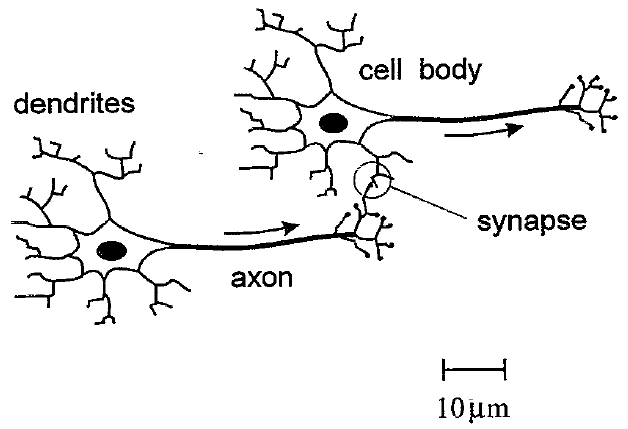
\includegraphics[width=0.8\textwidth]{brain.png}
   \caption{Esquema de las redes de neuronas en un cerebro humano. Tomada de [1].}
\end{figure}

El cerebro humano es la estructura más compleja conocida. Contiene alrededor de $10^{11}$ células activadas eléctricamente, denominadas neuronas. Como se representa el la Fig. 1, el árbol de dendritas proveé un conjunto de inputs a la neurona, mientras que el axón actúa como un output. Las neuronas se comunican entre sí a través de uniones llamadas sinapsis. Cada neurona típicamente se une a miles de otras neuronas, por lo que el número total de sinapsis excede $10^{14}$, y aunque cada neurona procesa la información de manera lenta (alrededor de 1 ms), el paralelismo masivo del conjunto de neuronas lleva a un poderoso procesamiento de información, mucho mayor al de supercomputadoras actuales.\\

Las neuronas actúan de una manera de ``todo o nada''. Cuando una neurona ``se acciona'' envía un impulso eléctrico que se propaga hasta la sinapsis. En ese momento se activa la liberación de neuro-transmisores químicos que se propagan hacia la siguiente célula. Dependiendo del tipo de sinapsis, se puede incrementar o disminuir la probabilidad de que una neurona subsecuente se accione. Cada sinapsis tiene asociado un peso que determina la magnitud del efecto del impulso en la siguiente neurona. Por lo tanto, cada neurona realiza una suma con pesos del input de otras neuronas, y si la suma total excede cierto límite entonces la neurona se activa.\\

Una propiedad clave para las NNs es su habilidad para modificar su respuesta ante señales externas. A esto se le conoce como \textit{learning}, y ocurre debido a cambios en la magnitud de la sinapsis.\\

\begin{figure}[th!]
   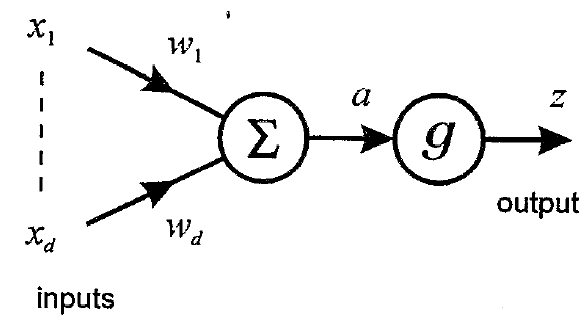
\includegraphics[width=0.85\textwidth]{unit.png}
   \caption{Modelo de McCuloch y Pitts de una única neurona. Tomada de [1].}
\end{figure}

En analogía al caso biológico, las NNs artificiales están compuestas por unidades de procesamiento (Fig. 2). Cada unidad ingresa $i$ datos de entrada (inputs), $x_i$, los cuales se multiplican por parámetros conocidos como pesos, $w_i$ (los cuales determinan la importancia de los inputs dados), para posteriormente, mediante la suma de estos inputs pesados, producir una señal de salida (output). Esto se representa matemáticamente por, 
\begin{equation}
    a=\sum^{d}_{i=1} w_i x_i + w_0,
\end{equation}
donde el parámetro $w_0$ es denominado \textit{bias}, y representa el límite de activación de una neurona bilógica. Formalmente, el bias puede incluirse como un caso especial de un peso correspondiente a un imput extra con valor $x_0=1$, por lo que se tiene,
\begin{equation}
    a=\sum^{d}_{i=0} w_i x_i.
\end{equation}
Nótese que los pesos (y el bias) pueden ser de cualquier signo, correspondiendo a sinapsis excitatorias o inhibitorias. El output, $z$, es finalmente dado por el valor de $a$, modulado por una \textit{función de activación}, $g()$,
\begin{equation}
   z=g(a). 
\end{equation}
Algunos ejemplos de funciones de activación se muestran en la Fig. 3.\\

\begin{figure}[th!]
   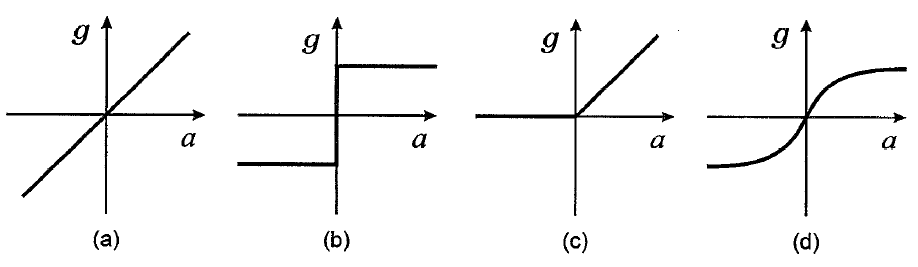
\includegraphics[width=0.95\textwidth]{act.png}
   \caption{Funciones de activación típicas: (a) lineal, (b) threshold, (c) threshold lineal, (d) sigmoidal. Tomada de [1].}
\end{figure}

Si el output excede un cierto umbral dado, entonces se activa el nodo, lo cual resulta en pasar el output de la actual unidad como input de la siguiente unidad en la red. Uniendo muchos elementos de procesamiento (layers) es posible construir NNs mas grandes y poderosas (multilayer), como se muestra en la Fig. 4 para el caso de dos unidades. En este caso si consideramos la primera unidad, tendremos outputs  en cada nodo dados por,
\begin{equation}
    z_j=g \left( \sum_{i=0}^d w_{ji} x_i\right),
\end{equation}
donde $w_{ji}$ denota el peso del input $i$ de la unidad $j$.\\

Los outputs de la NN se obtienen al proceder de la misma manera, pero ahora tomando en la segunda unidad de procesamiento como inputs a los valores $z_j$ procesados previamente por la primera unidad, de modo que los outputs $y_k$ estarán dados por
\begin{equation}
    y_k=\Tilde{g} \left( \sum_{j=0}^m \Tilde{w}_{kj} z_j\right),
\end{equation}
donde $\Tilde{w}_{kj}$ denota el peso en la segunda unidad conectando la unidad $j$ con el output $k$. Es posible combinar las Ecs. (4) y (5) para tener una expresión completa para la transformación,
\begin{equation}
    y_k=\Tilde{g} \left( \sum_{j=0}^m \Tilde{w}_{kj} g \left( \sum_{i=0}^d w_{ji} x_i\right)\right).
\end{equation}
Las funciones de activación $g$ y $\Tilde{g}$ aplicadas en la salida de cada unidad de procesamiento no son, en general, iguales.\\

\begin{figure}[th!]
   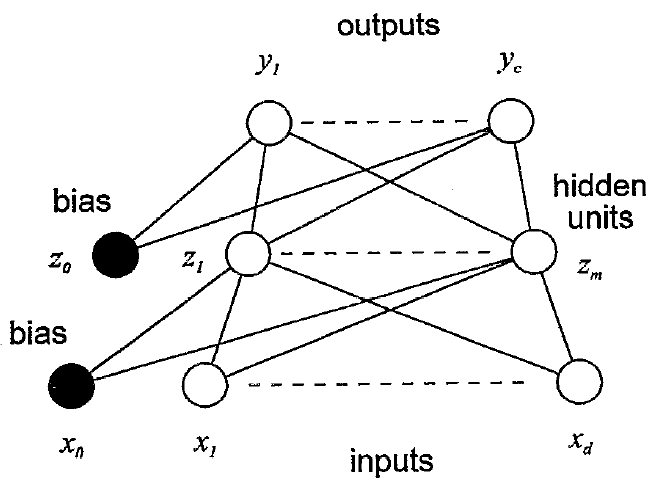
\includegraphics[width=0.85\textwidth]{two.png}
   \caption{NN de dos layers. Tomada de [1].}
\end{figure}

Note que en la Fig. 4 cada círculo debajo representa un input, cada círculo superior representa un output y cada peso entre ellos está representado por la linea que los une. Además, los círculos sólidos representan los parámetros de bias de cada input.\\

En la Fig. 5 se muestra una NN con múltiples layers (Deep NN). Es importante mencionar que las unidades de en medio se conocen como \textit{hidden units}, ya que sus valores de activación no son directamente accesibles desde fuera de la red.\\

\begin{figure}[th!]
   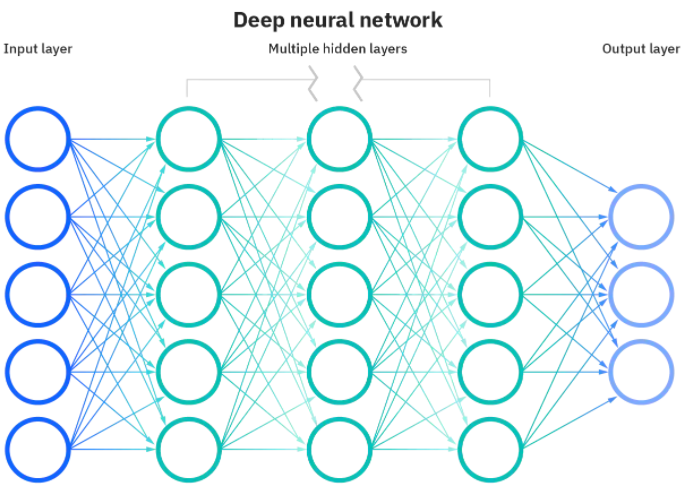
\includegraphics[width=0.95\textwidth]{deep.png}
   \caption{NN multilayer. Tomada de [2].}
\end{figure}

Un aspecto importante bien conocido es que para el entrenamiento de las NNs se requiere que la función de mapeo $y()$ sea diferenciable. Para esto, comunmente se utiliza la función de activacio sogmoidal (Fig. 3(d)), que para el caso de dos variables luce como la Fig. 6. Otras funciones de activación útiles en la práctica son ``tanh'' y ``logistic sigmoid'', dadas respectivamente por,
\begin{equation}
    g(a) = \frac{e^a -e^{-a}}{e^a +e^{-a}}
\end{equation}
y
\begin{equation}
    g(a) = \frac{1}{1 +e^{-a}}.
\end{equation}

\begin{figure}[th!]
   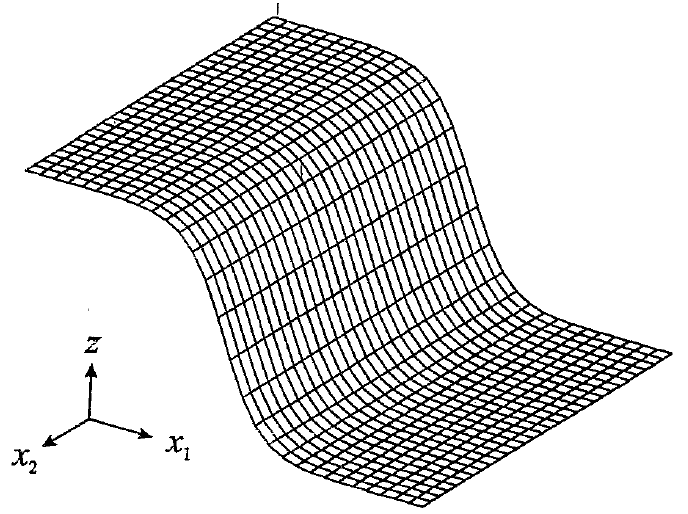
\includegraphics[width=0.8\textwidth]{sigm.png}
   \caption{Función de activación sigmoidal como función de dos variables input. Tomada de [1].}
\end{figure}

Cuando se comienza a pensar acerca de más usos prácticos de las NNs, tales como reconocimiento o clasificación de imágenes, es requerido un aprendizaje supervisado, esto es, por ejemplo, sets de datos con etiquetas (training set) para entrenar al algoritmo. Conforme evaluamos el algoritmo es deseable medir su precisión. Esto se evalúa comunmente por medio de una función de pérdida (\textit{loss}), que es típicamente calculada como el error cuadrático medio (MSE) entre los valores reales y los valores predichos,
\begin{equation}
    loss=MSE= \frac{1}{2m} \sum_{i=1}^m (\hat{y}-y)^2,
\end{equation}
donde $i$ es el índice de la muestra, $\hat{y}$ y $y$ son el resultado predicho y el resultado real, respectivamente, y $m$ es el número de muestras.\\

Finalmente, el objetivo es minimizar la función de pérdida para así tener un mejor encaje (fitting) de las predicciones. Para esto, el modelo ajusta sus pesos y bias para alcanzar un punto de convergencia en el error, o dicho de otra forma, un mínimo (local o global) de la función de pérdida. En la Fig. 7 se observa gráficamente el punto de convergencia para el caso de un solo input (peso) (a) y multiples inputs (pesos) (b).\\

\begin{figure}[th!]
   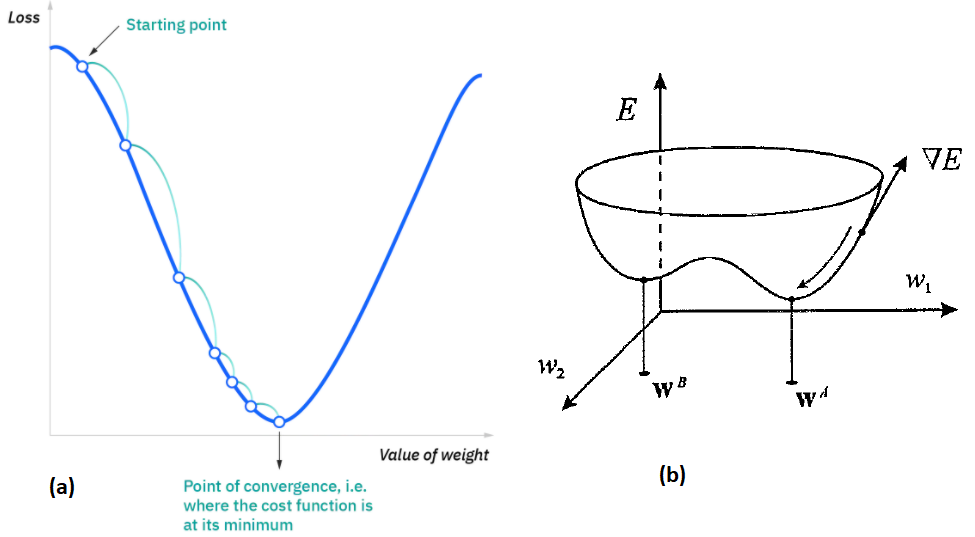
\includegraphics[width=0.95\textwidth]{loss.png}
   \caption{Función de pérdida. (a) Para el caso de un solo input. Tomada de [2]. (b) Para multiples inputs. El vector de peso $\mathbf{W}^A$ corresponde a un mínimo global de la funcion de pérdida, mientras que $\mathbf{W}^B$ representa un mínimo local. Tomada de [1].}
\end{figure}

Como se observa en la Fig. 7(b), el gradiente de la función de pérdida indica la dirección de máximo cambio de dicha función. Es posible icorporar un algoritmo denominado \textit{gradient descent algorithm} el cual, por medio de pequeñas modificaciones al vector de pesos, se mueve en la dirección opuesta a $\nabla E$, hasta que el vector de pesos alcanza un mínimo local o global.

\section{TensorFlow}
TensorFlow es una plataforma de código abierto total, desarrollada por Google, para la creación de aplicaciones de Machine Learning (ML) [3]. Es una librería matemática simbólica que utiliza dataflow y programación diferenciable para relizar varias tareas enfocado en el entrenamiento y la inferencia de deep NNs. Además, posee varias librerías, herramientas y fuentes comunitarias para un aprendizaje y uso más sencillo.

\subsection{¿Cómo funciona?}
TensorFlow te da la oportunidad de construir gráficos de flujo de datos (dataflow graphs), que es un conjunto de operaciones que toman lugar sucesivamente. Cada operación es conocida como \textbf{op node} y están conectadas unas a las otras. En una gráfica, cada nodo representa una operación matemática mientras que cada conección entre nodos es un tensor.

\subsection{¿Por qué es tan popular?}
Aquí enumeramos algunas razones por las cuales TensorFlow es tan popular:
\begin{enumerate}
    \item Ya que es totalmente open-source, TensorFlow contiene la mejor librería para desarrollo de aplicaciones de AI.
    \item La librería de TensorFlow integra varios APIs (Application Programming Interfaces) para construir arquitecturas de aprendizaje profundo.
    \item El marco de TensorFlow está basado en el cálculo de gráficos de flujo de datos, lo cual de la posibilidad a los desarrolladores de representar y monitorear el desarrollo de la NN.
    \item TensorFlow hace posible la depuración de aplicaciones.
    \item Como TensorFlow está construido en Python, es fácil de aprender e implementar.
    \item Tanto C++ como Python APIs están soportados por TensorFlow, lo cual hace que el desarrollo se mas sencillo que en otros marcos.
    \item Las librerías y paquetes incluyen miles de funciones construidas (built-in) que hace posible a los desarrolladores evitar escribir complejos y tardados códigos.
    \item Es posible usarse en otros lenguajes como Java o R, que están integrados con TensorFlow también.
    \item Es posible trabajar tanto con GPUs como con CPUs.
\end{enumerate}

\subsection{Arquitectura}
La arquitectura de un pograma en TensorFlow trabaja en tres partes:
\begin{itemize}
    \item Preprocesamiento de los datos: Declaración de variables, creación o importación de datos y preproceso de los mismos para su manejo mas fácil.
    \item Creación del modelo: Operaciones a desarrollar.
    \item Entrenamiento y estimación del modelo: Entrenamiento de la NN usando datos previamente cargados y estimación de la función de pérdida.
\end{itemize}

Una vez que se realizaron los pasos anteriores (fase de desarrollo), es posible utilizar el modelo para inferir resultados de datos nuevos (fase de inferencia).\\

Finalmente, una herramienta de gran utilidad es TensorBoard, que permite monitorear gráfica y visualmente lo que TensorFlow está haciendo.\\

A continuación se muestra un ejemplo de un modelo en TensorFlow para clasificar prendas de vestir.

\subsection{Ejemplo de NN en TensorFlow: clasificación de prendas de vestir}
Vamos a ver el ejemplo de clasificación de prendas de vestir utilizando un modelo en TensorFlow. Para ello seguiremos los siguientes pasos: Importar el set de datos; preprocesar el set de datos; construir el modelo; entrenar el modelo y evaluar su precisión; hacer predicciones.

\subsubsection{Importar el set de datos}
Se utiliza el set de datos ``Fashion MNIST'', el cual contiene 70 000 imágenes en escala de grises (Fig. 8) distribuidas en 10 categorías: 0: T-short/Top; 1: Trouser; 2: Pullover; 3: Dress; 4: Coat; 5: Sandal; 6: Shirt; 7: Sneaker; 8: Bag; 9: Ankle Boot. Éstas etiquetas son almacenadas en un tensor.

\begin{figure}[th!]
   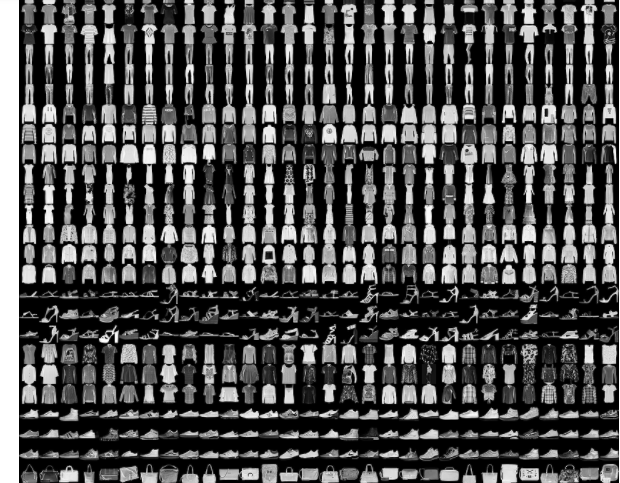
\includegraphics[width=\textwidth]{prendas.png}
   \caption{Imágenes de muestra del set de datos ``Fashion MNIST''.}
\end{figure}

A continuación se muestra el código que realiza estos pasos:

\begin{figure}[th!]
   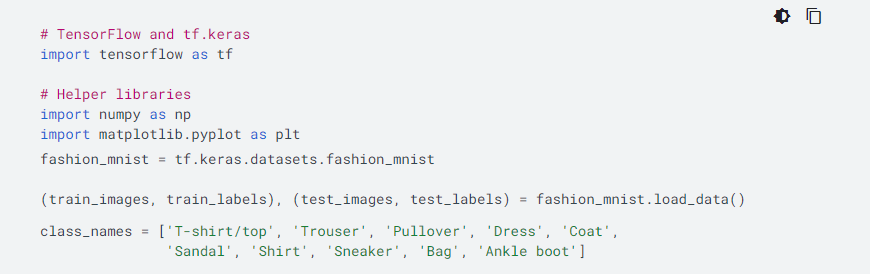
\includegraphics[width=\textwidth]{import.png}
\end{figure}

\subsubsection{Preprocesamiento de datos}
Las imágenes contienen valores de pixeles que van desde 0 a 255. Para utilizarlos en un modelo de NN se requiere que dichos valores vayan de 0 a 1, por lo que es necesario dividir los valores de los sets entre 255.0:

\begin{figure}[th!]
   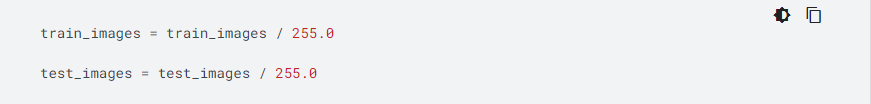
\includegraphics[width=\textwidth]{preproc.png}
\end{figure}

\subsubsection{Construcción del modelo}
La construcción del modelo requiere configurar sus layers y después proceder a compilarlo. Para la creación de los modelos se pueden utilizas diferentes APIs, sin embargo, la más usada en TensorFlow es ``keras''. A continuación se muestra el código para la creación del modelo:

\begin{figure}[th!]
   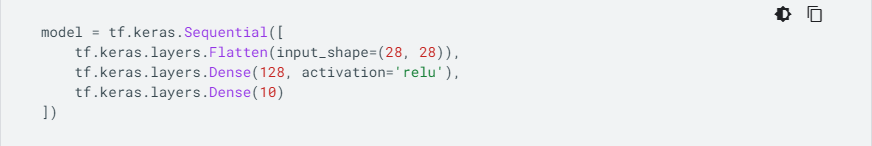
\includegraphics[width=\textwidth]{model.png}
\end{figure}

La capa ``Flatten'' transforma el formato de las imágenes de un tensor bidimensional de $28$ por $28$ pixeles a un tensor unidimensional de $28\cdot 28= 784$ pixeles. Por otro lado, las capas `` Dense'' consisten de capas totalmente conectadas de NNs, las cuales tienen parámetros que se aprenden durante el entrenamiento.\\

Para compilar el modelo es necesario agregar algunas configuraciones extras: La función de pérdida (loss), la cual se quiere minimizar; el optimizador (optimizer), que es cómo el modelo se actualiza basado en los datos de entrenamiento y la función de pérdida; y el parámetro metrics, el cual monitorea los pasos de entrenamiento y de prueba:

\begin{figure}[th!]
   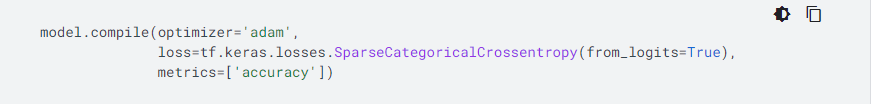
\includegraphics[width=\textwidth]{compile.png}
\end{figure}

\subsubsection{Entrenamiento y evaluación}
El entrenamiento de una NN requiere los siguientes pasos:
\begin{itemize}
    \item Darle los datos de entrenamiento al modelo. En este ejemplo estos datos son ``train\_images'' y ``train\_labels''.
    \item El modelo aprende a asociar imágenes con etiquetas. El parámetro ``epochs'' hace referenca al número de épocas durante as cuales se entrenará en modelo.
    \item Se pueden hacer predicciones, verificando la precisión del modelo:
    
\end{itemize}
\begin{figure}[th!]
   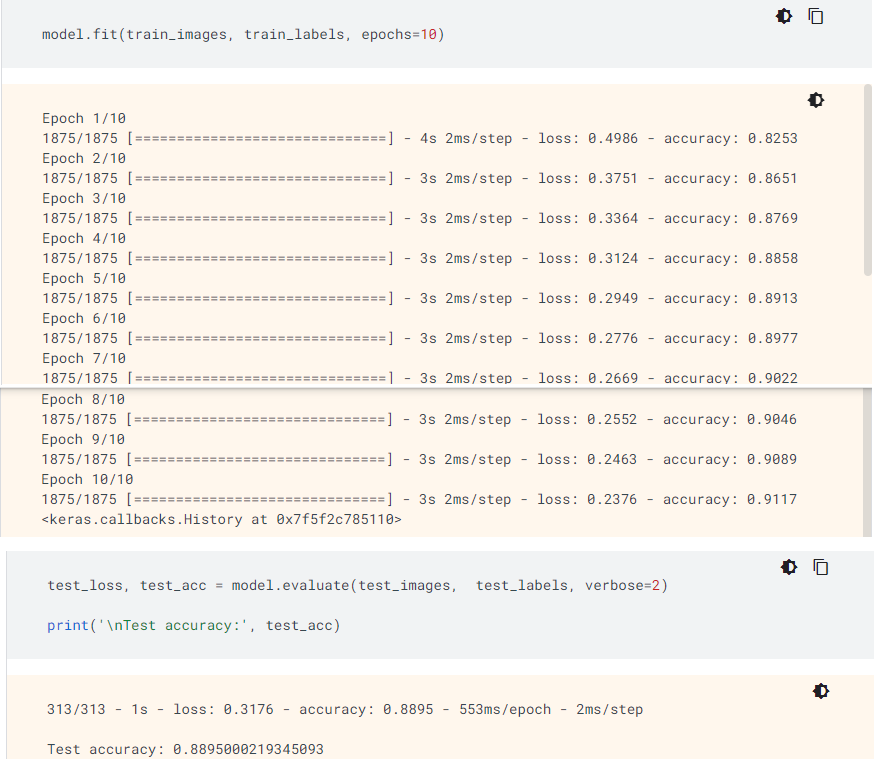
\includegraphics[width=\textwidth]{train.png}
\end{figure}

En este ejemplo se puede observar, desués de 10 épocas de entrenamiento, que la NN alcanza una precisión de 0.91, con un valor de la función de pérdida de 0.23, en el set de entrenamiento, mientras que para el set de prueba sus valores disminuyen a 0.89 y 0.32 para la precisión y la pérdida, respectivamente.

\subsubsection{Predicciones}
Con el modelo ya entrenado, es posible hacer predicciones acerca de imágenes de prueba. En el siguiente código se utiliza la capa ``softmax'' para convertir los outputs a probabilidades. Además, al hacer la predicción del elemento cero del tensor ``predictions'' se obtiene un array con las probabilidades de que su correspondiente etiqueta sea 0-10.

\begin{figure}[th!]
   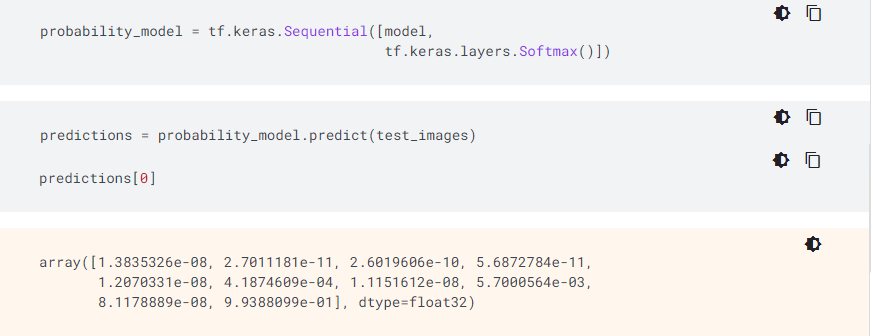
\includegraphics[width=\textwidth]{pred.png}
\end{figure}

Se observa que la etiqueta que tiene mayor probabilidad es la número 9, con un 99.3\% de probabilidad, correspondiente a un ``ankle boot''. Para visualizar esto de una mejor manera, se puede representar gráficamente la imágen con una gvráfica de probabilidades:

\begin{figure}[th!]
   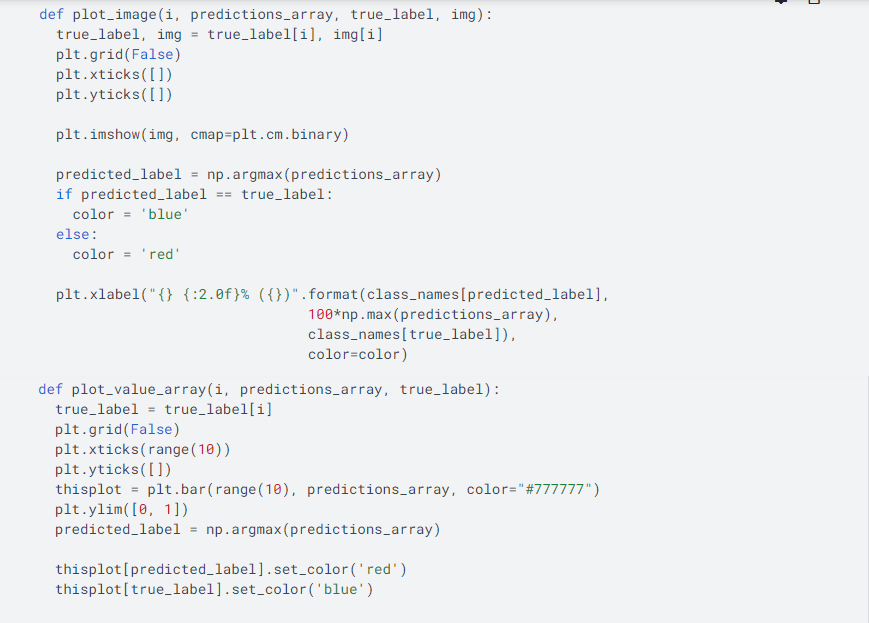
\includegraphics[width=\textwidth]{imag1.png}
\end{figure}
\begin{figure}[th!]
   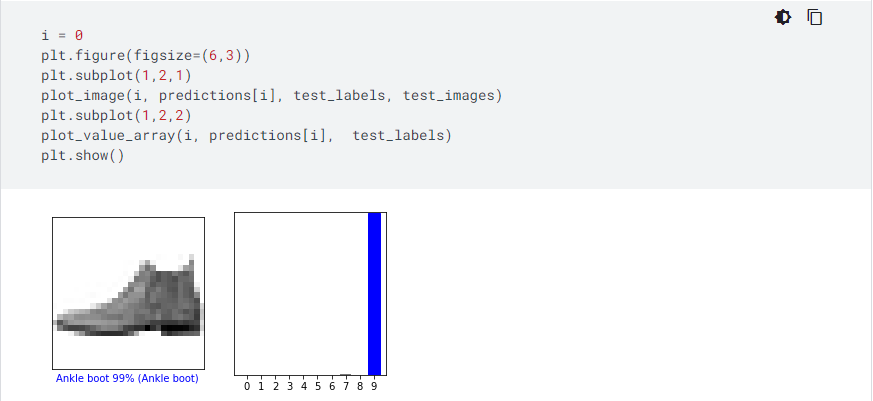
\includegraphics[width=\textwidth]{imag2.png}
\end{figure}

Se han definido funciones para graficar la imágen, así como un histograma con las probabilidades de que corresponda a la prenda 1-10.

\section{Trabajo en proceso y a futuro}
El propósito de los conocimientos adquiridos en este semestre que concluyó es aplicar le inteligencia artificial, en particular NNs, en el caso de las propiedades de transporte en grafeno. En particular, se busca generar un número de muestras suficientemente grande sobre perfiles de velocidad, conductividad, fuerza de arrastre, o alguna otra propiedad de transporte en los sistemas de grafeno con impurezas. Para tal propósito, se planea comenzar a desarrollar código para paralelizar los programas que realizan el cálculo hidrodinámico, mediante el uso del cluster del IFM. Una vez se tenga la base de datos suficiente, se utilizarán NNs para tratar de predecir comportamientos o configuraciones del sistema.\\

También, en los semestres que vienen se planea incluir campos externos a los cálculos.\\

Se ha realizado también en el semestre que concluyó, trabajo teórico en otros tipos de sistemas de Estado Sólido. En particular, se trabaja en cálculos teóricos del modelo SSH de aislantes topológicos y en el modelo de Jackiw y Rebbi. Se espera tener alguna publicación sobre ellos.

\section{Congresos y escuelas}
Es adecuado comentar que durante el periodo que comprende al semestre que concluyó, se tuvo la participación en el Congreso Nacional de Física 2022, organizado por la SMF, además de la escuela ``Topological Quantum Matter: Fundations and Applications'', organizada por la UNAM. Adicionalmente, se asistió al ``Curso Corto de Física de Materiales Bidimensionales'', organizado por el IPN.

\section*{Bibliografía}
[1] C. M. Bishop, Neural Networks and Their Applications, \textit{Rev. Sci. Instrum.} \textbf{65} (6) 1994. \newline
[2] https://www.ibm.com/cloud/learn/neural-networks \newline
[3] https://www.tensorflow.org/

\end{document}